\section{Topic 3. Interpolation and Polynomial Approximation}
\subsection{Defining Interpolation Problems}
Given a set of data points $\{(\mathbf{x}_i, \mathbf{y}_i)\}^n_{i=0} \subseteq \R^m \times \R^m$, we want to find a function $\mathbf{f}_n : \R^m \rightarrow \R^m$ so that $\mathbf{f}_n(\mathbf{x}_i) = \mathbf{y}_i$ for $0 \leq i \leq m$. For simplicity, we will first consider the case where $m = 1$.

\begin{marginfigure}
    In contrast to curve fitting, these equations are not satisfied exactly. They are satisfied in the least square sense.
\end{marginfigure}

\NewLine

\begin{defn}[Interpolant]
    Given a sequence of points $\{y_i\}_{i=0}^n$ sampled from an unknown function $f$, we call $f_n$ the \textbf{interpolant} of $f$.
\end{defn}

\NewLine

\noindent Our objective is to obtain the interpolant $f_n$ of $f$ and to evaluate it on data points that we have not yet observed. For instance,

\begin{center}
       
\includegraphics[width=0.8\textwidth]{figures/fig-4.png}
\end{center}

\begin{marginfigure}
    There are infinitely many ways to select the interpolant, so we will focus on choices of $f_n$ which have desirable approximation properties, e.g.,
    \begin{enumerate}
        \item Polynomials
        \item Piece-wise Polynomials
        \item Trigonometric Functions
    \end{enumerate}
\end{marginfigure}
\noindent  Since linear equations are easier to solve than non-linear ones, we will choose our interpolant to be a span by a set of functions,
\[f_n(x) = \sum_{i=1}^N c_j \cdot \phi_j(x)\]
where $\{\phi_j(x)\}_{j = 0}^N$ is a set of linearly independent \textbf{basis functions}.

\NewLine

\begin{defn}[Linear Independence]
    \sloppy A set of functions $\{\phi_j(x)\}_{j = 0}^N$ is called \textbf{linearly independent} on an interval $[a,b]$ if,
    \[\sum_{i=1}^N c_j \cdot \phi_j(x) = 0 \text{ on } [a,b] \quad \implies \quad c_j = 0  \quad \forall j \in [N]\]
    Otherwise, we call the set of functions \textbf{linearly dependent}.
\end{defn}

\NewLine

\noindent There are \textbf{three cases} to consider,
\begin{enumerate}
    \item If $N > n$, then $f_n$ exists but is not unique
    \item If $N < n$, then $f_n$ does not exist
    \item If $N = n$, then $f_n$ exists and is unique
\end{enumerate}

\noindent Suppose that we are given a set of data points $\{(x_i, y_i)\}_{i=0}^n$ on an interval $[a,b]$ of real numbers. With $\{\phi_j(x)\}_{j = 0}^N$ as a set of basis functions on $[a,b]$, observe that the coefficients $c_j$ satisfy that,
\[y_i = f_n(x_i) = \sum_{i=1}^N c_j \cdot \phi_j(x)\]
which we can write in matrix form as follows,
\[
\underbrace{\left(\begin{array}{cccc}
\phi_0\left(x_0\right) & \phi_1\left(x_0\right) & \ldots & \phi_n\left(x_0\right) \\
\phi_0\left(x_1\right) & \phi_1\left(x_1\right) & \ldots & \phi_n\left(x_1\right) \\
\vdots & \vdots & & \vdots \\
\phi_0\left(x_n\right) & \phi_1\left(x_n\right) & \ldots & \phi_n\left(x_n\right)
\end{array}\right)}_{:= \mathbf{A}}\left(\begin{array}{c}
c_0 \\
c_1 \\
\vdots \\
c_n
\end{array}\right)=\left(\begin{array}{c}
y_0 \\
y_1 \\
\vdots \\
y_n
\end{array}\right)
\]

\begin{rmk}
   $\mathbf{A}$ is invertible since $\left\{\phi_i(x)\right\}_{i=0}^N$ are basis functions, i.e., the columns of $\mathbf{A}$ are linearly independent.
\end{rmk}

\begin{defn}[Condition Number]
    \sloppy If $\mathbf{A}$ is invertible, then the \textbf{condition number} of $\mathbf{A}$ with respect to the matrix norm $\|\cdot\|$ is,
    \[\kappa(\mathbf{A}):=\|\mathbf{A}^{-1}\| \cdot \|\mathbf{A}\|\]
    Otherwise $\kappa(\mathbf{A}):= \infty$.
\end{defn}

\begin{rmk}
    For invertible $\mathbf{A}$, the condition number $\kappa(\mathbf{A})$ satisfies that,
    \begin{enumerate}
        \item If $\kappa(\mathbf{A}) = \kappa(\mathbf{A}^{-1}) $, then $1 \leq \kappa(\mathbf{A}) < \infty$ since
        \[\kappa(A)=\|A^{-1}\|\|A\| \geq\|A^{-1} A\|=1\]
        \item $\kappa(c\mA) = \kappa(\mA)$ for any constant $c \neq 0$
    \end{enumerate}
\end{rmk}

\begin{marginfigure}
    The norm of a matrix $\mA$ measures how much the mapping induced by that matrix can stretch vectors.
\end{marginfigure}


\begin{marginfigure}
    A matrix $\mA$ is singular if and only if its determinant $\text{det}(\mA)$ is 0.
\end{marginfigure}

\noindent $\mA$ is called \textbf{well-conditioned} if $\kappa(\mA)$ is close to 1 since small changes in $\mathbf{b}$ imply small changes in $\mathbf{x}$. Otherwise, $\mA$ is called \textbf{ill-conditioned} and small changes in $\mathbf{b}$ may result in large changes in $\mathbf{x}$.

\begin{ex}{Ill-Conditioned Matrices}{label}
    The following matrix is \textbf{ill-conditioned} in the $\ell_{\infty}$ norm.
    \begin{align*}
        &\mA=\left(\begin{array}{cc}
            0.123 & 0.456 \\
            0.789 & 2.92507
                \end{array}\right) \\
        &\mA^{-1}=-2.5641 \times 10^6\left(\begin{array}{cc}
            2.92507 & -0.456 \\
            -0.789 & 0.123
            \end{array}\right)
    \end{align*}
    We will compute $\|\mA\|_{\infty}$ and $\|\mA^{-1}\|_{\infty}$.
    \begin{align*}
    \|\mA\|_{\infty} &=\max \{0.123+0.456,0.789+2.92507\} \\
    &=\max \{0.579,3.71407\}=3.71407 \\
    \|\mA^{-1}\|_{\infty} &=2.5641 \times 10^6 \cdot \max \{2.92507+0.456,0.789+0.123\} \\
    &=2.5641 \times 10^6 \cdot \max \{3.3811,0.9120\}=8.6695 \times 10^6
    \end{align*}
    It follows that $\kappa(\mA) = \|\mA\|_{\infty} \cdot \|\mA^{-1}\|_{\infty} =3 .2199 \times 10^7$
\end{ex}

\begin{marginfigure}
    The value of $\kappa(\mA)$ depends on the matrix norm, but these are all technically related due to norm equivalences in $\R^n$.
    \begin{align*}
        &\|\mA\|_p=\sup _{x \neq 0} \frac{\|A x\|_p}{\|x\|_p} \\
        &\|\mA\|_1=\max _{1 \leq j \leq n} \sum_{i=1}^m\left|a_{i j}\right|\\
        &\|\mA\|_{\infty}=\max _{1 \leq i \leq m} \sum_{j=1}^n\left|a_{i j}\right|
    \end{align*}
\end{marginfigure}

\begin{marginfigure}
    If $\mA$ and $\mB$ are matrices and $x$ is a vector, then the following hold,
    \begin{align*}
        &\|\mA \mB\| \leq\| \mA \|\| \mB\| \\
        &\|\mA x\| \leq\|\mA\|\|x\|
    \end{align*}
    
\end{marginfigure}
\subsection{Monomial Basis Functions}
Consider a set of data points $\{(x_i, y_i)\}_{i=0}^n$. We want the interpolant to be a degree $n$ polynomial $f_n(x)=\sum_{j=0}^n c_j x^j$, so the first natural choice of basis functions is the \textbf{monomial basis} $\phi_j(x)=x^j$ for $j \in [n]$. The resulting linear system for interpolation is then,
\[
\underbrace{\left(\begin{array}{ccccc}
1 & x_0 & x_0^2 & \ldots & x_0^n \\
1 & x_1 & x_1^2 & \ldots & x_1^n \\
\vdots & \vdots & \vdots & & \vdots \\
1 & x_n & x_n^2 & \ldots & x_n^n
\end{array}\right)}_{:= \mV}\left(\begin{array}{c}
c_0 \\
c_1 \\
\vdots \\
c_n
\end{array}\right)=\left(\begin{array}{c}
y_0 \\
y_1 \\
\vdots \\
y_n
\end{array}\right)
\]
which is called the \textbf{Vandermonde matrix}.

\begin{rmk}
    In general, $\mV$ is \textbf{ill-conditioned} since,
    \[\text{det}(\mV) = \prod_{i \neq j}\left(x_i-x_j\right) \approx 0 \text { if any } x_i \approx x\]
    which implies $\kappa(\mA) \rightarrow \infty$. The proof is by induction, using the fact that $\operatorname{det} \mA=a_{11} \cdot \operatorname{det}(\mA_{11})+ a_{12} \cdot \operatorname{det}(\mA_{12}) +\ldots+a_{1 n} \cdot \operatorname{det}(\mA_{1 n})$
\end{rmk}

\noindent This motivates our study of the \textbf{Lagrange basis functions}.

\begin{marginfigure}
    The \textbf{Kronecker's delta} $\delta_{i j}$ is defined,
    \[\delta_{i j}= \begin{cases}1 & i=j \\ 0 & i \neq j\end{cases}\]
\end{marginfigure}

\subsection{Lagrange Basis Functions}
Consider a set of data points $\{(x_i, y_i)\}_{i=0}^n$. The \textbf{Lagrange basis functions} $\left\{\ell_j(x)\right\}_{j=0}^n$ are the $n$-th order polynomials satisfying,
\[\ell_j\left(x_i\right)=\delta_{j i}=\left\{\begin{array}{l}
0, \text { if } j \neq i \\
1, \text { if } j=i
\end{array}\right.\]
with the corresponding linear system, \[\underbrace{\left(\begin{array}{cccc}
1 & 0 & \ldots & 0 \\
0 & 1 & & 0 \\
\vdots & & \ddots & \vdots \\
0 & 0 & \ldots & 1
\end{array}\right)}_{\mA}\left(\begin{array}{c}
c_0 \\
c_1 \\
\vdots \\
c_n
\end{array}\right)=\left(\begin{array}{c}
y_0 \\
y_1 \\
\vdots \\
y_n
\end{array}\right) \Rightarrow c_i=y_i\]
for interpolation. The matrix $\mA$ is \textbf{well-conditioned} with $\kappa(\mA) = 1$. We will see two types of Lagrange basis functions,
\begin{enumerate}
    \item Linear Lagrange Polynomials
    \item Quadratic Lagrange Polynomials
\end{enumerate}

\begin{marginfigure}
    \begin{center}
    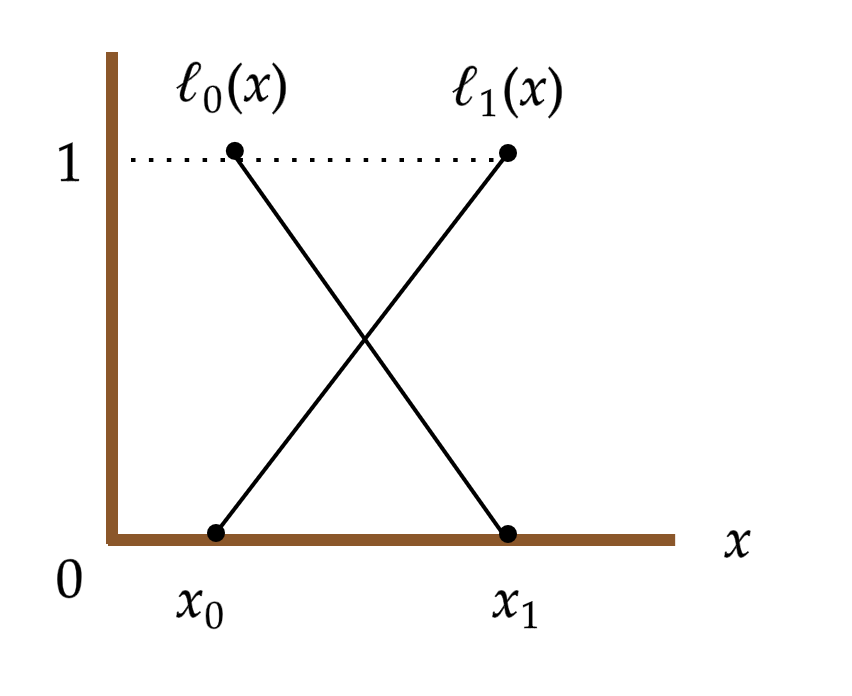
\includegraphics[width=\textwidth]{figures/fig-9.png}
    \end{center}
\end{marginfigure}

\noindent Suppose that $n = 1$. We will define the \textbf{linear Lagrange polynomial}. Given $\{x_0, x_1\}$, we want to find linear polynomials $\ell_0(x)$ and $\ell_1(x)$ so that $\ell_j\left(x_i\right)=\delta_{j i}$. Without loss of generality, let $\ell_0(x)=c\left(x-x_1\right) \text { so that } \ell_0\left(x_1\right)=0$. Thus, $1=\ell_0\left(x_0\right)=c\left(x_0-x_1\right)$ and,
\begin{align*}
    &\ell_0(x)=\frac{x-x_1}{x_0-x_1} \\
    &\ell_1(x)=\frac{x-x_0}{x_1-x_0}
\end{align*}

\noindent \sloppy Suppose that $n = 2$. We will define the \textbf{quadratic Lagrange polynomial}. Given $\{x_0, x_1, x_2\}$, we want to find $\ell_0(x)$, $ \ell_1(x)$, and $ \ell_2(x)$ so that $\ell_i\left(x_i\right)=\delta_{i i}$. As in the linear case, we set $\ell_0(x)=c\left(x-x_1\right)\left(x-x_2\right)$ to obtain that $\ell_0\left(x_1\right)=0=\ell_0\left(x_2\right)$. This gives $1=\ell_0\left(x_0\right)=c\left(x_0-x_1\right)\left(x_0-x_2\right)$ and therefore,
\begin{align*}
    &\ell_0(x)=\frac{\left(x-x_1\right)\left(x-x_2\right)}{\left(x_0-x_1\right)\left(x_0-x_2\right)} \\
    &\ell_1(x)=\frac{\left(x-x_0\right)\left(x-x_2\right)}{\left(x_1-x_0\right)\left(x_1-x_2\right)} \\
    &\ell_2(x)=\frac{\left(x-x_0\right)\left(x-x_1\right)}{\left(x_2-x_0\right)\left(x_2-x_1\right)}
\end{align*}

\begin{marginfigure}
    \begin{center}
    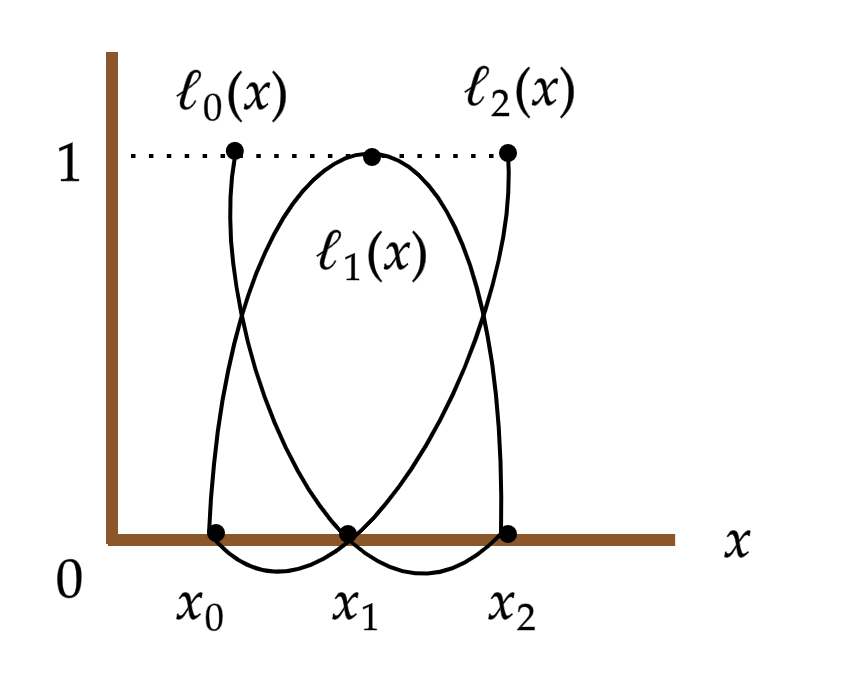
\includegraphics[width=\textwidth]{figures/fig-10.png}
    \end{center}
\end{marginfigure}

\begin{thm}[Lagrange Basis Formulas]
   \noindent Given a sequence $\left\{x_i\right\}_{i=0}^n$, the $j$-th \textbf{Lagrange basis function} is the $n$-th degree polynomial,
   \begin{align*}
       \ell_j(x)&=\frac{\left(x-x_0\right) \cdots\left(x-x_{j-1}\right)\left(x-x_{j+1}\right) \cdots\left(x-x_n\right)}{\left(x_j-x_0\right) \cdots\left(x_j-x_{j-1}\right)\left(x_j-x_{j+1}\right) \cdots\left(x_j-x_n\right)}
   \end{align*}
   which gives the interpolant,
   \[f_n = \sum_{j=0}^n y_j \ell_j(x) = \sum_{j=0}^n y_j \cdot \prod_{\substack{0 \leq k \leq n \\ k \neq j}} \frac{x-x_k}{x_j-x_k}\]
\end{thm}

\begin{proof}
    Check that $\ell_i\left(x_i\right)=\delta_{i i}$.
\end{proof}

\begin{ex}{Lagrange Interpolation}{label}
    We want to find the Lagrange polynomial for $\{(0,5),(1,4),(3,-2)\}$. Let \text{$x_0 = 0$}, \text{$x_1 = 1$}, and \text{$x_2 = 3$}. Then,
    \[f_2(x)=y_0 \ell_0(x)+y_1 \ell_1(x)+y_2 \ell_2(x) = \frac{1}{3}\left(-2 x^2-x+15\right)\]
    Observe that $f_n$ interpolates on these three points,
    \begin{align*}
        &f_2(0)=\frac{15}{3}=5 \\
        &f_2(1)=\frac{-2-1+15}{3}=\frac{12}{3}=4 \\
        &f_2(3)=\frac{-18-3+15}{3}=\frac{-6}{3}=-2
        \end{align*}
    \begin{center}
    
\includegraphics[width=\textwidth]{figures/fig-11.png}
    \end{center}
\end{ex}